% !TEX root = ../discretemath.tex

\section{BEST-теорема}

\subsection{Постановка}

Пусть $G$ — \textbf{сильно связный эйлеров орграф}: $\mathrm{indeg}(v)=\mathrm{outdeg}(v)$ для всех $v$.

\begin{Definition}{Арборесценция}{}
	\textbf{Арборесценцией с корнем $v$} (ориентированным остовным деревом, направленным к корню) называется подграф на $V(G)$, в котором из каждой вершины $u\neq v$ выходит ровно одно ребро и из любой вершины существует ориентированный путь в $v$. Обозначение: $t_v=\#\{\text{арборесценций с корнем }v\}$.
\end{Definition}

\begin{center}
	\begin{tikzpicture}[->,>=stealth,scale=0.85,
		every node/.style={circle,draw,minimum size=18pt,inner sep=0}]
		\node (v) at (0,0) {$v$};
		\node (a) at (-2.3,0.9) {$a$};
		\node (b) at (-2,-1) {$b$};
		\node (c) at (2.2,1) {$c$};
		\node (d) at (2.2,-0.9) {$d$};
		\node (e) at (4,0) {$e$};
		\draw (a)--(v); \draw (b)--(v); \draw (c)--(v);
		\draw (d)--(c); \draw (e)--(d);
		\node[draw=none,below=10pt] at (0,-1) {\small Арборесценция с корнем $v$};
	\end{tikzpicture}
\end{center}

\begin{Example}{}{}
	Полный симметричный орграф $K_3^{\leftrightarrow}$ на $\{1,2,3\}$ с рёбрами в обе стороны между всеми парами.
	\begin{center}
		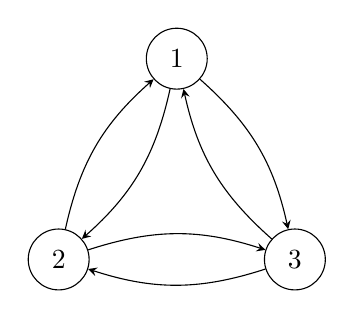
\begin{tikzpicture}[->,>=stealth,
			every node/.style={circle,draw,minimum size=22pt,inner sep=0}]
			\node (1) at (0,1.7) {$1$};
			\node (2) at (-1.5,-0.85) {$2$};
			\node (3) at (1.5,-0.85) {$3$};
			\draw[bend left=18] (1) to (2); \draw[bend left=18] (2) to (1);
			\draw[bend left=18] (2) to (3); \draw[bend left=18] (3) to (2);
			\draw[bend left=18] (1) to (3); \draw[bend left=18] (3) to (1);
		\end{tikzpicture}
	\end{center}
	Арборесценции с корнем $1$: $\{2{\to}1,3{\to}1\}$, $\{2{\to}1,3{\to}2\}$, $\{2{\to}3,3{\to}1\}$. Значит, $t_1=3$.
\end{Example}

\subsection{Формулировка}

\begin{Theorem}{BEST}{best}
	Пусть $G$ — сильно связный эйлеров орграф. Для любого $v\in V(G)$:
	\[
	\mathrm{ec}(G)=t_v\cdot\prod_{u\in V(G)}\bigl(\mathrm{outdeg}(u)-1\bigr)!,
	\]
	где $\mathrm{ec}(G)$ — число эйлеровых циклов с фиксированным первым ребром, исходящим из $v$.
\end{Theorem}

\begin{Corollary}{}{}
	В сильно связном эйлеровом орграфе $t_u=t_v$ для всех $u,v$ (правая часть не зависит от выбора корня).
\end{Corollary}

\begin{Remark}{}{}
	$t_v$ вычисляется по матричной теореме Кирхгофа для орграфов: $t_v=\det(\widetilde L_v)$, где $\widetilde L_v$ — лапласиан $G$ без строки и столбца вершины $v$. Частный случай (одна вершина, ноль рёбер): $\mathrm{ec}(G)=1=1\cdot 0!=1$.
\end{Remark}

Число эйлеровых \emph{путей}, начинающихся в $v$ (в эйлеровом орграфе каждый замкнут, то есть является циклом):
\[
\#\text{Эйл. путей из }v=\mathrm{outdeg}(v)\cdot\mathrm{ec}(G).
\]

\subsection{Доказательство}

\subsubsection*{Цель и идея}

Достаточно установить
\begin{equation}\label{eq:goal}
	\#\text{Эйл. путей из }v
	=t_v\cdot\mathrm{outdeg}(v)!\cdot\!\!\prod_{u\neq v}\!\bigl(\mathrm{outdeg}(u)-1\bigr)!
	=\mathrm{outdeg}(v)\cdot\mathrm{ec}(G).
\end{equation}
Строим биекцию между $\mathcal A$ — эйлеровыми путями из $v$ — и $\mathcal B$ — парами $(T,\sigma)$, где $T$ — арборесценция с корнем $v$, а $\sigma$ — упорядочение исходящих рёбер каждой вершины, в котором ребро из $T$ стоит \emph{последним} для $u\neq v$ (для $v$ — любой порядок). Тогда $|\mathcal B|=t_v\cdot\mathrm{outdeg}(v)!\cdot\prod_{u\neq v}(\mathrm{outdeg}(u)-1)!$.

\subsubsection*{Шаг 1. Эйлеров путь порождает арборесценцию}

Для пути $P$ возьмём для каждого $u\neq v$ \emph{последнее} исходящее из $u$ ребро $e_u$ как дерево-ребро; $\sigma$ — порядок использования рёбер в $P$.

\begin{Statement}{}{}
	Рёбра $\{e_u\}_{u\neq v}$ образуют арборесценцию с корнем $v$.
\end{Statement}

\begin{proof}
	Их ровно $|V|-1$ (по одному из каждой $u\neq v$); достаточно показать отсутствие цикла. Пусть, от противного, есть цикл $C=a_1\to\cdots\to a_k\to a_1$, $v\notin C$.

	\begin{center}
		\begin{tikzpicture}[->,>=stealth,bend angle=25,
			every node/.style={circle,draw,minimum size=20pt,inner sep=0}]
			\node (a1) at (0,0) {$a_1$};
			\node (a2) at (2.2,1.1) {$a_2$};
			\node[fill=red!15] (aj) at (5,1.1) {$a_j$};
			\node (ajp) at (7.2,0) {$a_{j\!+\!1}$};
			\draw (a1) to (a2);
			\draw[dotted,thick] (a2) to (aj);
			\draw[thick,red!70!black] (aj) to (ajp);
			\node[draw=none,above=5pt,font=\footnotesize,red!70!black] at (6.1,0.65) {шаг $m$ (макс.)};
			\draw (ajp) to[bend right=38] (a1);
		\end{tikzpicture}
	\end{center}

	Пусть $a_j$ — вершина $C$, чьё дерево-ребро $e_{a_j}$ использовано под максимальным номером $m$ среди рёбер вершин цикла. После шага $m$ путь в $a_{j+1}$. Так как $m$ максимально, ребро $e_{a_{j+1}}$ (последнее исходящее из $a_{j+1}$) использовано раньше — значит, все исходящие из $a_{j+1}$ уже израсходованы, и путь не может продолжиться, хотя $a_{j+1}\neq v$. Противоречие с полнотой эйлерова пути.
\end{proof}

\subsubsection*{Шаг 2. Упорядочение порождает эйлеров путь}

По $(T,\sigma)$ строим путь: в вершине $u$ берём первое по $\sigma(u)$ ещё не использованное исходящее ребро.

\begin{Statement}{}{}
	Построенный путь эйлеров.
\end{Statement}

\begin{proof}
	\textbf{Путь заканчивается в $v$.} Ходьба не может остановиться в $u\neq v$: если все $\mathrm{outdeg}(u)$ рёбер из $u$ использованы, а ходьба завершилась в $u$, то заходов в $u$ на $1$ больше выходов, что невозможно при $\mathrm{indeg}(u)=\mathrm{outdeg}(u)$. Значит, ходьба кончается в $v$.

	\textbf{Разбиение.} Пусть $A=\{u:\text{все исходящие из }u\text{ пройдены}\}$, $B=V\setminus A$. Тогда $v\in A$. Предположим $B\neq\varnothing$.

	\begin{center}
		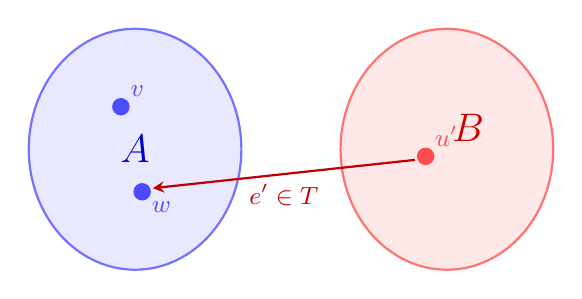
\begin{tikzpicture}[scale=0.9]
			\draw[blue!55,thick,fill=blue!9] (-2.2,0) ellipse (1.5cm and 1.7cm);
			\node[blue!80!black,font=\Large\bfseries] at (-2.2,0) {$A$};
			\fill[blue!70] (-2.4,0.6) circle (3.5pt) node[above right,font=\small,draw=none]{$v$};
			\fill[blue!70] (-2.1,-0.6) circle (3.5pt) node[below right,font=\small,draw=none]{$w$};
			\draw[red!55,thick,fill=red!9] (2.2,0) ellipse (1.5cm and 1.7cm);
			\node[red!80!black,font=\Large\bfseries] at (2.5,0.3) {$B$};
			\fill[red!70] (1.9,-0.1) circle (3.5pt) node[above right,font=\small,draw=none]{$u'$};
			\draw[->,>=stealth,thick,red!75!black] (1.75,-0.15) -- (-1.95,-0.55)
			node[midway,below,font=\small,draw=none]{$e'\in T$};
		\end{tikzpicture}
	\end{center}

	\textbf{Подсчёт переходов.} (1) Все рёбра из $A$ пройдены, поэтому $\#$переходов $A{\to}B=\#$рёбер $A{\to}B$. (2) Ходьба начинается и кончается в $v\in A$, поэтому $\#$переходов $A{\to}B=\#$переходов $B{\to}A$. (3) В эйлеровом орграфе $\#$рёбер $A{\to}B=\#$рёбер $B{\to}A$. Из (1)–(3): $\#$переходов $B{\to}A=\#$рёбер $B{\to}A$, то есть все рёбра $B\to A$ пройдены.

	\textbf{Противоречие.} В арборесценции $T$ (все пути ведут к $v\in A$) найдётся $u'\in B$, чьё дерево-ребро $e'=(u',w)$ ведёт в $A$. Ребро $B\to A$ пройдено, но $e'$ — последнее в $\sigma(u')$, значит, все рёбра из $u'$ пройдены и $u'\in A$ — противоречие с $u'\in B$.
\end{proof}

\subsubsection*{Итог}

Шаги 1–2 дают взаимно обратные отображения $\mathcal A\leftrightarrow\mathcal B$ — биекцию. Из~\eqref{eq:goal}:
\[
\mathrm{ec}(G)=\frac{\#\text{Эйл. путей из }v}{\mathrm{outdeg}(v)}
=\frac{t_v\cdot\mathrm{outdeg}(v)!\cdot\prod_{u\neq v}(\mathrm{outdeg}(u)-1)!}{\mathrm{outdeg}(v)}
=t_v\cdot\prod_{u\in V(G)}(\mathrm{outdeg}(u)-1)!.
\]
